
% --------------------------------------------------------------- CONFIGURATIONS

%ifdef TWOSIDE
	%\documentclass[a4paper,12pt,final,twoside,openright]{book}
%elif ONESIDE
	\documentclass[a4paper,12pt,final,oneside]{book}
%endif

\usepackage{rapport}


% -------------------------------------------------------------- META: CONSTANTS

\newcommand{\reporttitle}{Prolog}
\newcommand{\enseignants}{Jean~François~\textsc{Boulicaut}\\ Mehdi~\textsc{Kaytoue}}
\newcommand{\reportauthor}{Guillaume~\textsc{Abadie}\\ Nicolas~\textsc{Buisson}\\ Louise~\textsc{Crépet}\\ Rémi~\textsc{Domingues}\\ Aline~\textsc{Martin}\\ Martin~\textsc{Wetterwald}}
\newcommand{\hexanome}{H4404}
\newcommand{\reportsubject}{Livrable de projet}
\newcommand{\stagetopic}{Puissance 4}
\newcommand{\dateperiod}{du 1\up{er} au 15 octobre 2013}
\newcommand{\HRule}{\rule{\linewidth}{0.5mm}}
\setlength{\parskip}{1ex} % Espace entre les paragraphes

\hypersetup{
	pdftitle={\reporttitle},%
		pdfauthor={\reportauthor},%
		pdfsubject={\reportsubject},%
		pdfkeywords={INSA Lyon} {Prolog} {Puissance 4}
}

\title{\reporttitle}
\author{\reportauthor}
%\setcounter{tocdepth}{4}


% ------------------------------------------------------------------------- FILE

\begin{document}


    % ------------------------------------------------------------------- HEADER

	\renewcommand{\chaptername}{} %\renewcommand{\thechapter}{}

	\pagestyle{empty}
	\pagenumbering{Roman}


    % ------------------------------------------------------------ HEADER: TITLE

	% Inspiré de http://en.wikibooks.org/wiki/LaTeX/Title_Creation
\begin{center}
	\begin{minipage}[t]{0.48\textwidth}
	  \begin{flushleft}
	    
\includegraphics [width=40mm]{images/logo_INSA.png} \\[0.5cm]
			INSA Lyon\\
			20, avenue Albert Einstein\\
			69621 Villeurbanne Cedex
	  \end{flushleft}
	\end{minipage}
	\begin{minipage}[t]{0.48\textwidth}
	  \begin{flushright}
	    %\includegraphics [width=60mm]{images/logo_Passau.jpg} \\[0.5cm]
	    %Universität Passau\\
		%Innstraße, 3\\
		%	D-94032 Passau
	  \end{flushright}
	\end{minipage} \\[2cm]

	\textsc{\Large \reportsubject}\\[0.3cm]
	\HRule \\[0.4cm]
	{\Huge \bfseries \reporttitle}\\[0.3cm]
	{\LARGE \bfseries «~\stagetopic~»}\\[0.3cm]
	{\Large \dateperiod}\\[0.4cm]
	\HRule \\[1cm]

	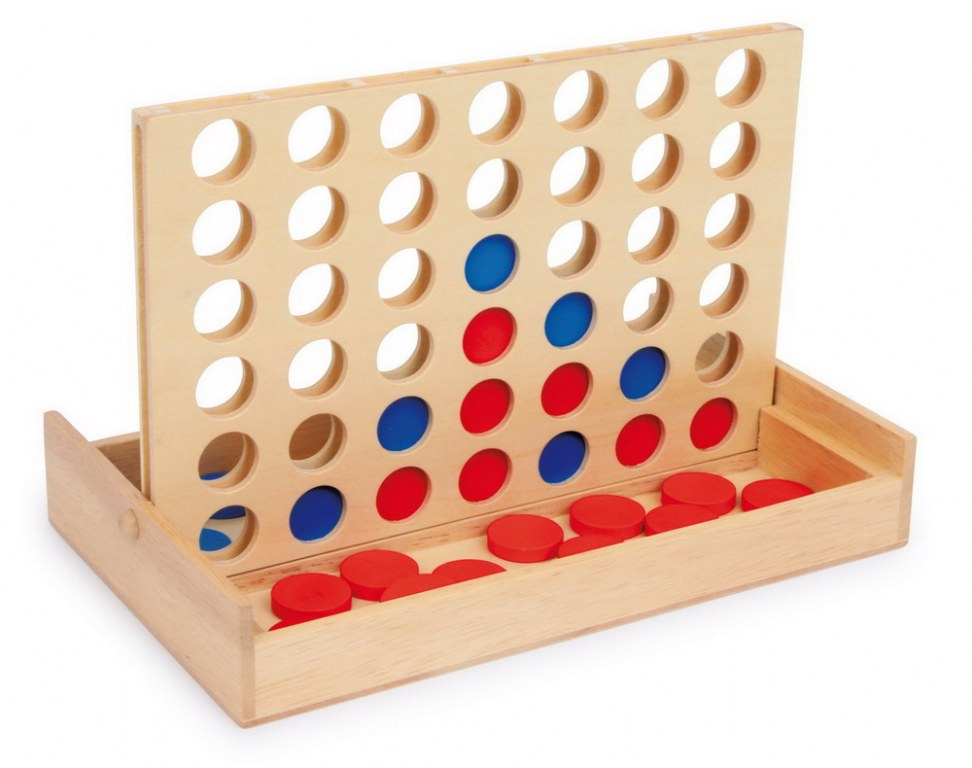
\includegraphics [scale=0.25]{images/puissance4.jpg} \\[0.7cm]
	\begin{minipage}[t]{0.4\textwidth}
	  \begin{flushleft} \large
	    \emph{Hexanôme \textbf{\hexanome}~:}\\
	    \small \reportauthor
	  \end{flushleft}
	\end{minipage}
	\begin{minipage}[t]{0.5\textwidth}
	  \begin{flushright} \large
	    \emph{Enseignants~:} \\
	    \enseignants
	  \end{flushright}
	\end{minipage}

	\vfill
	\footnotesize{Année scolaire 2013-2014}
\end{center}


	%ifdef TWOSIDE
		%\cleardoublepage
	%endif

	%% Inspiré de http://en.wikibooks.org/wiki/LaTeX/Title_Creation
\begin{center}
	\vspace*{8cm}
	\textsc{\Large \reportsubject}\\[0.3cm]
	\HRule \\[0.4cm]
	{\Huge \bfseries \reporttitle}\\[0.3cm]
	{\LARGE \bfseries «~\stagetopic~»}\\[0.3cm]
	{\Large \dateperiod}\\[0.4cm]
	\HRule \\[1cm]

	\begin{minipage}[t]{0.4\textwidth}
	  \begin{flushleft} \large
	    \emph{Hexanôme \textbf{\hexanome}~:}\\
	    \small \reportauthor
	  \end{flushleft}
	\end{minipage}
	\begin{minipage}[t]{0.5\textwidth}
	  \begin{flushright} \large
	    \emph{Enseignants~:} \\
		\enseignants
	  \end{flushright}
	\end{minipage}
\end{center}


	%ifdef TWOSIDE
		%  \newpage
		%	\null
		%	\vfill
	%endif


    % --------------------------------------------------- HEADER: CONFIGURATIONS

	\sloppy          % Justification moins stricte : des mots ne dépasseront pas des paragraphes



	\mainmatter
	\pagestyle{headings}

	\renewcommand{\chaptermark}[1]{\markboth{\MakeUppercase{\chaptername\ \thechapter.\ #1}}{}}
	\renewcommand{\sectionmark}[1]{\markright{\thesection{} #1}}


    % ------------------------------------------------------------------ CONTENT

    
\chapter{Bilan des éxercices}

\section{Predicats}

La particularite Prolog reside dans le fait qu'il n'y a plus d'iterations comme
un language de programmation conventionnel. Tout n'est que predicat. Ainsi, la
methode de programmation change de facon de penser. Fini le traitement de donnes
dans des variable que l'on met jour, car la programmation predicat permet
simplement de lier des proprietes entre des variables et/ou constantes.

Considerons pour la suite, le predicat :
\[(membre(X, L) \Leftrightarrow vrai) \Leftrightarrow X \in L\]


\section{Vérification de propriétés}

La vérification de propriétés permet s'assurer que une (out plusieur) constantes
verifies un ensemble de predicat. Considerons le code ci dessous :

Alors on a à l'éxécution :

\begin{lstlisting}[language=Prolog]
?- membre(1, [1, 2, 3]).
true

?- membre(4, [1, 2, 3]).
false
\end{lstlisting}

En effet, a la premiere intérogation, on vérifie le prédicat $1 \in [1, 2, 3]$
ce qui est vrai, d'ou la reponse de Prolog 'vrai'. La proprieté etre ces deux
paramêtres est alors vérifié, renvoyant ainsi vrai. Tandis que la seconde
interogation $4 \in [1, 2, 3]$ est fausse car $4 \notin [1, 2, 3]$, d'ou la
reponse 'false'.


\section{Reprouvabilitée}

La reprouvabilitees consiste maintenant de definir des propriete entre des
variables et/ou constantes. Par exemple :
\begin{center}
$X \in [1, 2, 3]$.
\end{center}

 Ce qui en Prolog donne :
\begin{lstlisting}[language=Prolog]
?- membre(X, [1, 2, 3]).
\end{lstlisting}

On lis a ce moment que $X$ compose la liste constante $[1, 2, 3]$. Ainsi a
l'execution, Prolog peut evaluer les solutions de $L$ grace a cette proprietee
ainsi définie :

\begin{lstlisting}[language=Prolog]
?- membre(L, [1, 2, 3]).
L = 1;
L = 2;
L = 3;
false
\end{lstlisting}


\section{Reprouvabilitée multiple}

Une propriétée sur une variable par exemple, peut etre definit par plusieur
predicats. Par exemple~:
\[
    \left\{  
    \begin{array}{c}
        L \in [1, 2, 3]\\
        L \in [3, 4, 2]\\
    \end{array}
    \right .
\]

Cela revient simplement a l'ecriture en Prolog :
\begin{lstlisting}[language=Prolog]
?- membre(L, [1, 2, 3]), membre(L, [3, 4, 2]).
L = 2;
L = 3;
false
\end{lstlisting}


\section{Reprouvabilitée non-déterministe}

La dangeureusitee de de la reprouvabilitée, est qu'il est possible qu'une
infinitée de solutions vérifient une meme propriétée. Considerons par exemple
le code suivant~:

\begin{lstlisting}[language=Prolog]
?- membre(1, L).
\end{lstlisting}

Cette est equivalent à $1 \in L$. Mais alors, combien de listes
pourraient vérifié cette propriété ?

\textbf{Initialisation}~: Une liste telle que $[1, 2]$ vérifie cette propriété.

\textbf{Hérédité}~: En notant $cat(A, B)$ la concatenation de deux listes $A$ et
$B$,\\
Soit une liste $L$ telle que $1 \in L$,\\
Alors $\forall X \in \mathbb{N} / 1 \in cat([X], L)$

\textbf{Conclusion}~: Il éxiste une infinité de solutions et Prolog va essayer
de toutes les générer, causant une exception du au manque de mémoire de la
machine.

\begin{lstlisting}[language=Prolog]
?- membre(1, L).
L = [1|_G2214] ;
L = [_G2213, 1|_G2217] ;
L = [_G2213, _G2216, 1|_G2220] ;
L = [_G2213, _G2216, _G2219, 1|_G2223] ;
L = [_G2213, _G2216, _G2219, _G2222, 1|_G2226] ;
L = [_G2213, _G2216, _G2219, _G2222, _G2225, 1|_G2229] ;
...
\end{lstlisting}


\section{Programation de prédicats}

Au paravant, nous fesions que utiliser des prédicats, mais bien entendu,
l'objectif est de pouvoir coder les siens. Pour cela, interessons nous a la
reecriture de
\[(membre(X, L) \Leftrightarrow vrai) \Leftrightarrow X \in L\]

\begin{lstlisting}[language=Prolog]
membre(X, [X|_]).
membre(X, [_|L]) :- membre(X, L).
\end{lstlisting}


	\chapter{Projet~: Puissance~4}

\section{Règles du jeu}
Le \texttt{Puissance~4} est un jeu de société à deux joueurs. Chaque joueur doit,
chacun son tour, insérer un jeton de sa couleur dans une des sept colonnes
du plateau de jeu, chacune ayant une capacité maximale de six jetons. On peut voir chaque colonne comme
une pile de jetons, puisqu'on ne peut qu'empiler des jetons les uns sur les autres.
Le but du jeu est d'\textbf{aligner} verticalement, horizontalement ou en diagonale \textbf{4~jetons} de sa couleur avant l'adversaire.


\section{But du joueur idéal}

Dans le cas d'un joueur idéal, le but est simplement, après avoir aligné 3~jetons,
de prévoir de jouer le 4\up{ème} au tour suivant. Mais, comme l'adversaire pourrait casser la ligne en jouant à cet endroit
lors de son tour, l'objectif du joueur idéal est donc de réaliser au moins deux alignements de 3 jetons,
laissant ainsi le joueur adverse contre l'inévitable~: il ne pourra plus contrer ces alignements en un seul jeton.


\section{Travail réalisé}

En plus de l'implémentation du module du mécanisme de jeu et de la réalisation des
tests unitaires, nous avons implémenté 4 joueurs autonomes, dont une intelligence artificielle~:
\begin{itemize}

    \item joueur aléatoire~;
    \item joueur aléatoire muni d'heuristiques~;
    \item joueur parcourant l'arbre des possibilités~;
    \item intelligence artificielle apprenant par \textbf{moteur d'inférence} de ses
    échecs précédents.\\
\end{itemize}

Mais également~:
\begin{itemize}
    \item interface utilisateur en ligne de commande pour jouer une partie~;
    \item module de tournois générant des statistiques~;
    \item module d'entrainement du moteur d'inférence~;
    \item module d'étude de l'apprentissage du moteur d'inférence~;
    \item sauvegarde et chargement de la base de connaissances du moteur d'inférence.
\end{itemize}



    % ------------------------------------------------------------------- FOOTER
\end{document}
